\documentclass[10pt,letterpaper]{article}

\usepackage{cvpr}
\usepackage{times}
\usepackage{epsfig}
\usepackage{graphicx}
\usepackage{amsmath}
\usepackage{amssymb}
\usepackage{wrapfig}
\usepackage[breaklinks=true,bookmarks=false]{hyperref}
\cvprfinalcopy

\begin{document}

%%%%%%%%% TITLE
\title{\textsf{Advanced Algorithms project Report}}

\author{Giacomo Fabris\\
University of Trento\\
{\tt\small giacomo.fabris-1@studenti.unitn.it}
}

\maketitle
%\thispagestyle{empty}

\section{Introduction}

%-------------------------------------------------------------------------
Objective of the project is to create a classifier which is able to determine which illness (if any) affects the lungs of a patient, based on their thoracic X-rays images. Illnesses shall be classified in 4 categories: none, bacterial infection, COVID-19, viral infection (non-COVID).

The dataset on which the classifier is trained is composed of about 6000 samples, made of (a) the black-white thoracic X-rays image, 256 pixel wide and high, and (b) a feature vector of 84 entries, extracted from the image.

\section{Proposed Method}

I considered the use of neural networks to solve the classification task, performing two main experiments:
\begin{enumerate}
    \item using as input the feature vectors only, I implemented a simple feed-forward neural network;
    \item using as input both the pictures and the feature vectors, I implemented a (small) deep neural network.
\end{enumerate}

\subsection{Feed-forward network on feature vectors}

The feed-forward neural network is composed of 4 layers of, respectively, 84, 42, 21 and 4 perceptron.
Increasing further the number of layers had no sensible effect on the precision of the model; similarly, the effect of changing the number of perceptrons of each hidden layer was not dramatic, above a certain threshold.

I experimented with two optimizers, Stochastic Gradient Descent and Adagrad. (...)

As a mean to control overfitting, I considered both dropout layers and weight decays (L2 regolarizers)...


\subsection{Deep network on image dataset}

\begin{wrapfigure}{r}{0.25\textwidth}
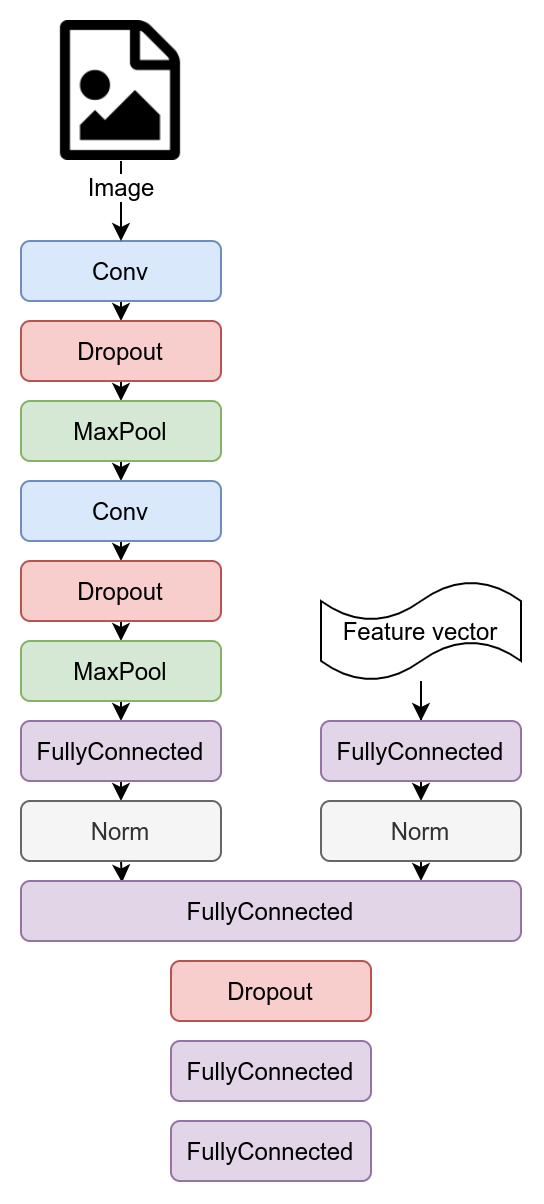
\includegraphics[width=0.9\linewidth]{Network.png}
\caption{Deep network structure}
\end{wrapfigure}

I considered these methods... I noticed these advantages... I noticed these disadvantages ...

The final solution...

\section{Results}

I have implemented the approach with... and performed the following experiments... 

%{\small
%\bibliographystyle{ieee}
%\bibliography{egbib}
%}

\end{document}
